\chapter{Diseño de la interfaz de explicaciones}
\label{cap:interfaz}

El objetivo de nuestro proyecto, como ya hemos expresado anteriormente en este documento, consiste en proporcionar explicaciones que justifiquen la relación existente entre dos canciones proporcionadas por un recomendador de música. Una vez realizado el estudio de las canciones y las distintas explicaciones posibles, es necesario mostrar el resultado de nuestro estudio de una forma gráfica, comprensible para un usuario humano.\\

Los datos que manejamos en nuestro estudio consisten en objetos y las relaciones que existen entre ellos, pues siguen el modelo de datos RDF. Necesitamos representar todos los caminos que se forman entre las dos canciones iniciales, mostrando las conexiones existentes entre los objetos intermedios. Por estos motivos hemos decidido llevar a cabo la visualización mediante un grafo porque consideramos que se adecúa mejor a nuestras necesidades.\\

Es importante que la interfaz sea fácil de entender y usar, así que siempre trataremos de mantenerla lo más sencilla posible. La base de nuestro diseño es el grafo de explicaciones ya mencionado, pues es el elemento más importante debido a la gran cantidad de información que aporta y, por lo tanto, es también la parte central de la interfaz alrededor de la cual se posicionarán el resto de elementos.\\

\section{Diseño del grafo}

\begin{figure}[h!]
	\centering
	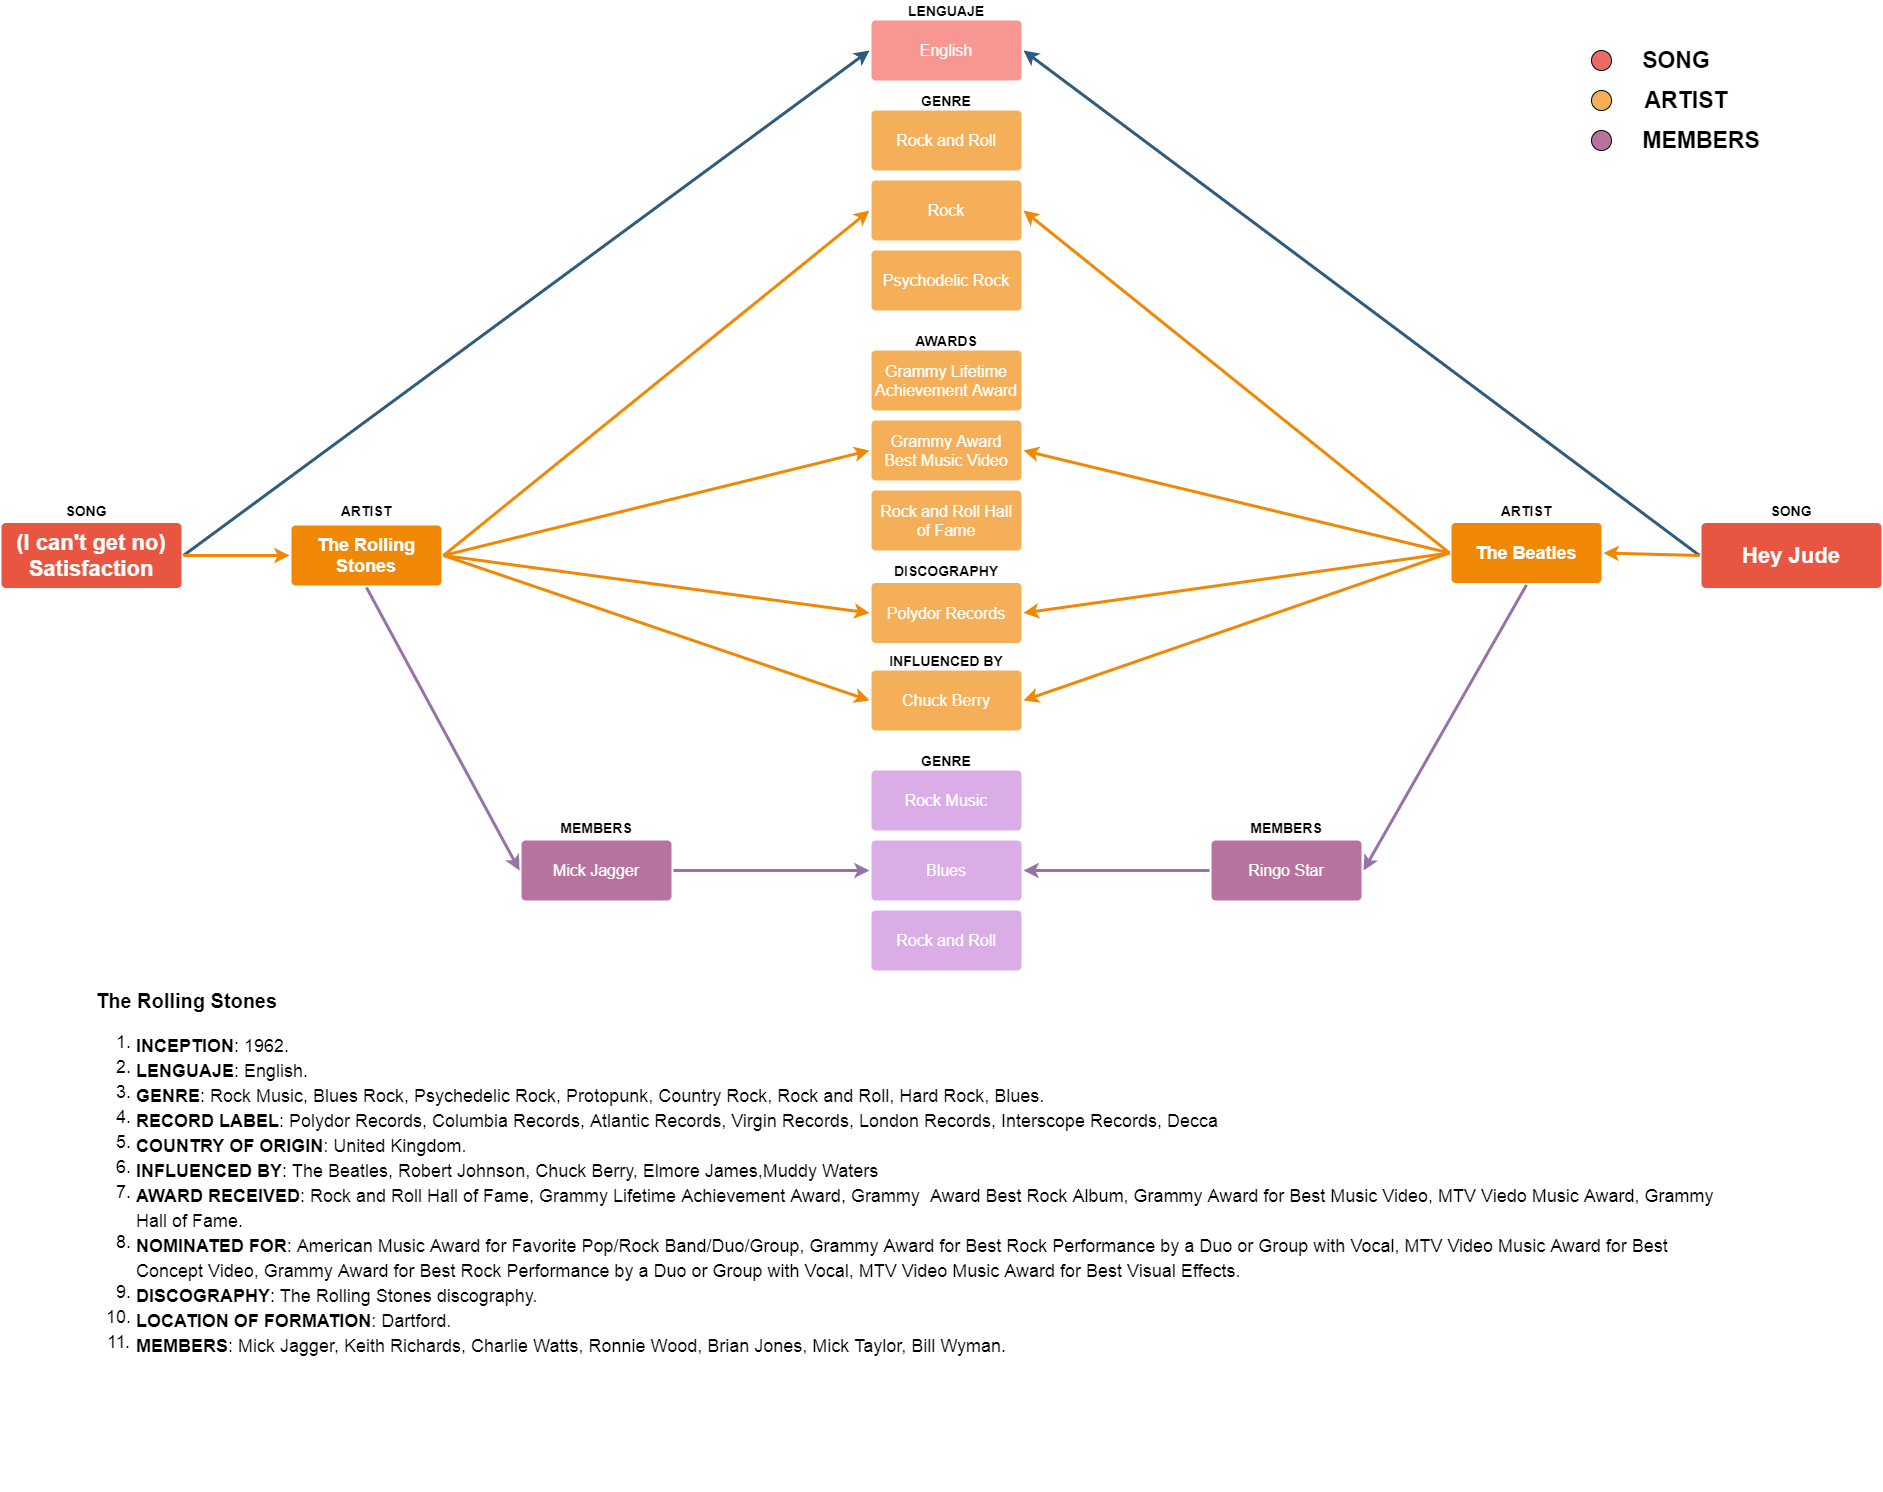
\includegraphics[width = 1\textwidth]{Imagenes/Bitmap/InterfaceResult.png}
	\caption{Primer diseño de la interfaz web}
	\label{fig:sampleImage}
\end{figure}

En la Figura 4.1 se puede observar la primera iteración de nuestro diseño. En ella se ve un ejemplo de grafo donde los nodos son los distintos sujetos y objetos (según el modelo RDF), mientras que las aristas representan los predicados que relacionan a esos nodos.\\

Los nodos posicionados a ambos extremos son las canciones sobre las que estamos realizando el estudio, diferenciados por el color rojo. A partir de ellas parten todas las explicaciones. En el centro se puede ver también un nodo coloreado de un rojo más suave, este representa al objeto de una explicación directa (en este caso la explicación ``Idioma'').\\

Los nodos coloreados de color naranja representan los artistas de ambas canciones y las relaciones que existen entre ellos, de la misma forma que en el anterior caso con las canciones y las explicaciones directas. Estas explicaciones obtenidas por el estudio de los artistas son indirectas, ya que requieren un estudio más profundo para relacionar las canciones originales.\\

Por último tenemos nodos morados que representan a los miembros o integrantes de los artistas, pues en este caso dichos artistas son bandas formadas por varias personas. Su funcionamiento es el mismo que el descrito en el párrafo anterior, con la salvedad de que estos miembros se obtienen del artista y, por lo tanto, sus explicaciones presentan un nivel extra de profundidad.\\

En esta versión del diseño también se propone una funcionalidad que permite visualizar datos adicionales. Haciendo click en los nodos sobre los que se hacen los estudios (canciones, artistas y miembros), se despliega una sección inferior en la que se muestran todos los datos obtenidos en el estudio del elemento concreto, aparezcan en el grafo o no. Así podemos ver todos los sellos discográficos con los que trabajaron \textbf{The Rolling Stones} aunque solo \textbf{Polydor Records} los relacione con \textbf{The Beatles}.\\

Esta función no es integral para el objetivo de nuestro proyecto, tan solo es un complemento que ofrece opciones al usuario. Por ello se le ha dado una prioridad baja durante el desarrollo de este trabajo y acabó siendo retirado de diseños posteriores por carecer del interés suficiente para la materia que nos ocupa.\\

\section{Diseño de la interfaz}

Pasaremos ahora a explicar el resto de la interfaz con la ayuda de la Figura 4.2. En esta iteración, el diseño del grafo se mantiene intacto en la mayor parte. Las novedades a destacar es que se pueden ver las explicaciones indirectas obtenidas por el estudio de los géneros de la canción, representados por nodos de color verde, además de que el nombre de las explicaciones (el predicado según RDF) se traslada a las aristas. (WIP. SEGURAMENTE HAYA QUE CAMBIAR ESTE PÁRRAFO Y/O LA IMAGEN)\\

\begin{figure}[h!]
	\centering
	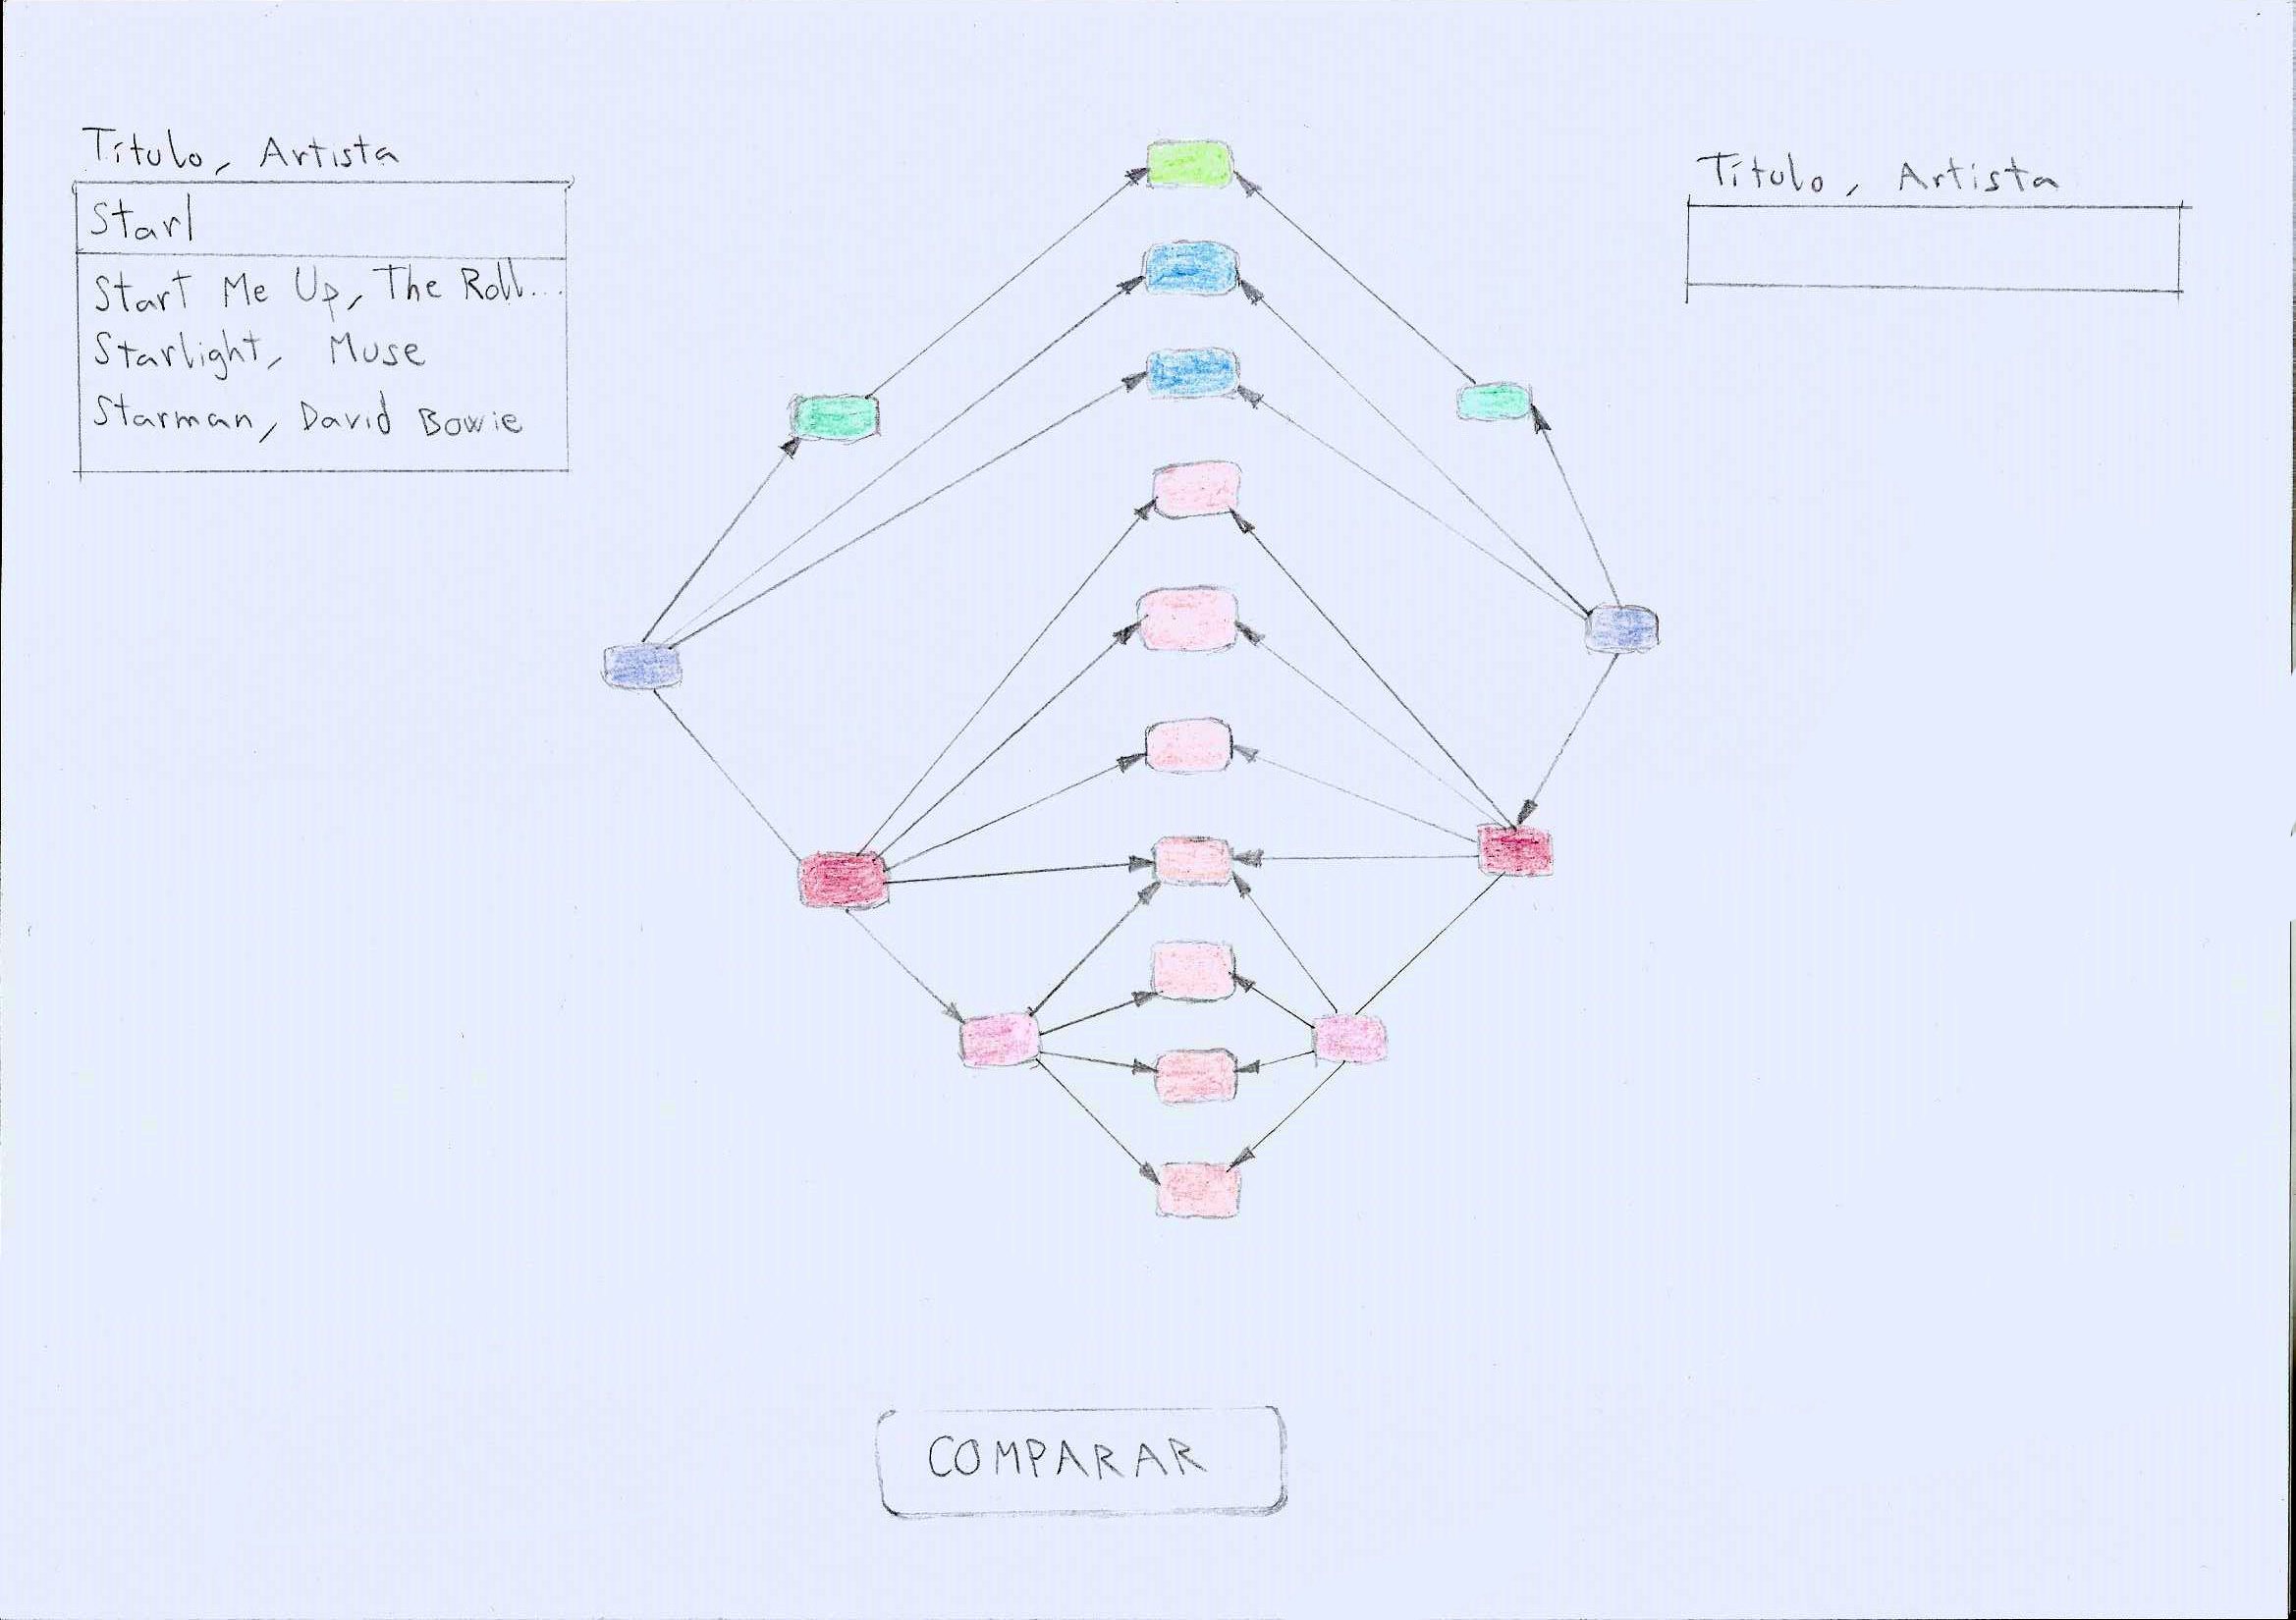
\includegraphics[width = 0.9\textwidth]{Imagenes/Bitmap/Segunda Interfaz.jpg}
	\caption{Primer diseño de la interfaz web}
	\label{fig:sampleImage}
\end{figure}

El resto de la interfaz consiste en los elementos con los que interactuará el usuario antes de generar el grafo de explicaciones. A ambos lados de la pantalla se sitúan los campos a rellenar con los datos básicos de las canciones. Para identificar la canción deseada es necesario escribir en ellos el título de la canción y el nombre de su artista, separados por una coma. En realidad este campo de entrada es un buscador que mostrará en un desplegable la lista de canciones que coinciden con el texto introducido y el usuario deberá seleccionar la que está buscando. Si intenta comparar una canción no contemplada por el sistema, aparecerá un mensaje de error.\\

La decisión de limitar las posibles entradas ha sido tomada por motivos prácticos. En Wikidata hay una cantidad ingente de temas musicales registrados, sin embargo los datos de cada canción concreta no siempre son tan completos como cabría esperar. A menudo falta información o la que hay no aparece siguiendo los mismos estándares que el resto, especialmente cuando se trata de canciones menos populares. Por ello hemos elaborado una lista de canciones que poseen información útil en Wikidata y que podemos tratar en nuestra aplicación sin problemas.\\

Por último, en la parte inferior de la pantalla hay un botón para ``COMPARAR’’. Una vez rellenados los campos de las dos canciones con opciones válidas, el usuario deberá pulsar este botón para que se dibuje el grafo de explicaciones. La primera vez que se use la aplicación no aparecerá ningún grafo en el centro de la interfaz, pero en las comparaciones siguientes el grafo previo no se borrará hasta pulsar de nuevo este botón para dibujar un grafo nuevo.\\
